\documentclass{beamer}
\usepackage{amsfonts,amsmath,oldgerm}
\usetheme{dmpisa} % Here the call to the beamer theme

\usepackage[english]{babel}
\usepackage{hyperref}
\usepackage{media9}
\usepackage{multimedia}
\usepackage{graphicx}
\usepackage{animate}
\usepackage{subfig}
%\usepackage{enumitem}
\usepackage[font=scriptsize]{caption}
\captionsetup[subfigure]{labelformat=empty}



%Per stile dei teoremi, delle definizioni, etc...
\theoremstyle{definition}
\newtheorem{dfn}{Definizione}[section]
\newtheorem{es}{Esempio}[section]
\newtheorem{oss}{Osservazione}[section]
\newtheorem{ese}{Esercizio}[section]
\theoremstyle{plain}
\newtheorem{thm}{Teorema}[section]
\newtheorem{cor}{Corollario}[section]
\newtheorem{lem}{Lemma}[section]
\newtheorem{prop}{Proposizione}[section]

%%
\newcommand{\testcolor}[1]{\colorbox{#1}{\textcolor{#1}{test}}~\texttt{#1}}
\usefonttheme[onlymath]{serif}
\titlebackground*{assets/background}
\newcommand{\hrefcol}[2]{\textcolor{cyan}{\href{#1}{#2}}}

\title{HLT Project: Progress Update}
\subtitle{Sentiment Analysis on Amazon Reviews}
\vspace{0.3cm}
\course{HLT - Group 11}
%\vspace{0.3cm}
\author{\href{mailto:a.nardone5@studenti.unipi.it}{Angelo Nardone}, \href{mailto:r.marcaccio@studenti.unipi.it}{Riccardo Marcaccio}, \href{mailto: m.ziboli@studenti.unipi.it}{Matteo Ziboli}}
\date{April 18, 2024}

\begin{document}
\maketitle

\footlinecolor{maincolor}

%~~~~~~~~~~~~~~~~~~~~~~~~~~~~~~~~~~~~~~~~~~~~~~~~~~~~~~~~~~~~~~~~~~~~~~~~~
\begin{frame}{Introduction}
\framesubtitle{HLT Project: Progress Update}
{\small 
\begin{itemize}

    \item We already discussed the two datasets we'll be utilizing for our project and outlined our objectives. 

    \item We've delved deeper into our datasets. 

    \item We will now see how we handled the following parts:
    \begin{enumerate}
        \item \textcolor{teal}{Data Loading}
        \item \textcolor{teal}{Data Cleaning}
        \item \textcolor{teal}{Data Analysis}
    \end{enumerate}

    \item The next step is to start working on our classification task using machine learning.
\end{itemize}
}
\end{frame}


%~~~~~~~~~~~~~~~~~~~~~~~~~~~~~~~~~~~~~~~~~~~~~~~~~~~~~~~~~~~~~~~~~~~~~~~~~~~~~~~~~~~~~~~~
%~~~~~~~~~~~~~~~~~~~~~~~~~~~~~~~~~~~~~~~~~~~~~~~~~~~~~~~~~~~~~~~~~~~~~~~~~~~~~~~~~~~~~~~~
\section{Data Loading}


%~~~~~~~~~~~~~~~~~~~~~~~~~~~~~~~~~~~~~~~~~~~~~~~~~~~~~~~~~~~~~~~~~~~~~~~~~
\begin{frame}{Using Pandas}
\framesubtitle{HLT Project: Data Loading}
{\small 
\begin{columns}
    \column{0.5\textwidth}
    \begin{itemize}
        \item Used \texttt{Pandas} to handle the data.
        \item Loaded both datasets using the command \texttt{pd.read\_csv()}.
        \item Quickly saw the contents of the datasets.
    \end{itemize}

    \column{0.5\textwidth}
    \begin{figure}
        \centering
        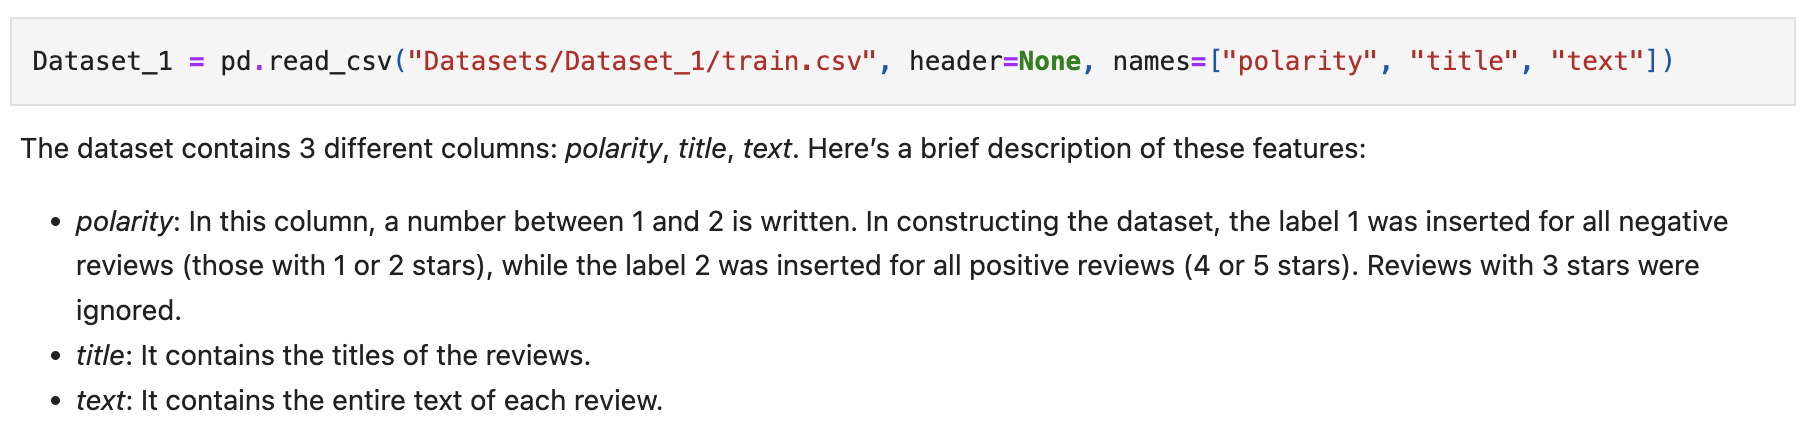
\includegraphics[scale=0.23]{Figures/read2.png}
    \end{figure}
\end{columns}

\begin{columns}
    \column{0.5\textwidth}
        \begin{figure}
        \centering
        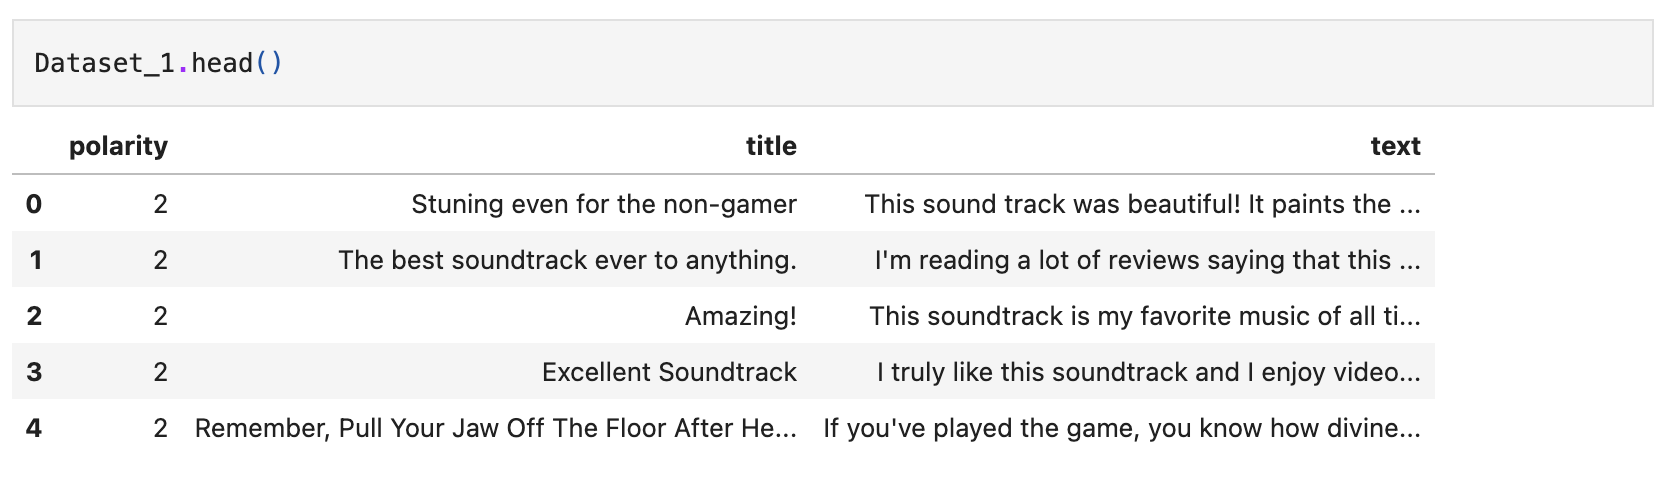
\includegraphics[scale=0.25]{Figures/head.png}
    \end{figure}

    \column{0.5\textwidth}
        \begin{figure}
        \centering
        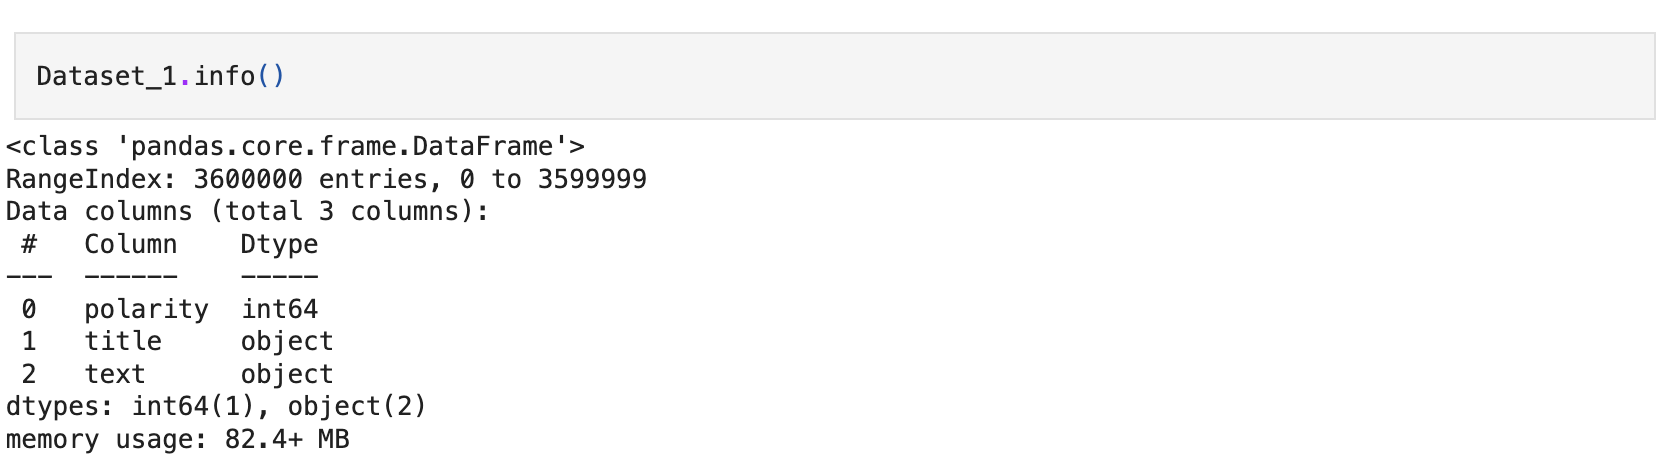
\includegraphics[scale=0.25]{Figures/info.png}
    \end{figure}
\end{columns}
}
\end{frame}

%~~~~~~~~~~~~~~~~~~~~~~~~~~~~~~~~~~~~~~~~~~~~~~~~~~~~~~~~~~~~~~~~~~~~~~~~~~~~~~~~~~~~~~~~
%~~~~~~~~~~~~~~~~~~~~~~~~~~~~~~~~~~~~~~~~~~~~~~~~~~~~~~~~~~~~~~~~~~~~~~~~~~~~~~~~~~~~~~~~
\section{Data Cleaning}

%~~~~~~~~~~~~~~~~~~~~~~~~~~~~~~~~~~~~~~~~~~~~~~~~~~~~~~~~~~~~~~~~~~~~~~~~~
\begin{frame}{Duplicated Rows and Null Values}
\framesubtitle{HLT Project: Data Cleaning}
{\small 

\begin{itemize}
    \item The datasets were already quite clean.
    \item We had to do only a few operations.
\end{itemize}

\vspace{0.2cm}
\begin{columns}
    \column{0.5\textwidth}
    \textbf{Dropping Duplicated Rows}

     \begin{itemize}
         \item We eliminated duplicate rows, keeping one occurrence per row.
     \end{itemize}

    \column{0.5\textwidth}
    \begin{figure}
        \centering
        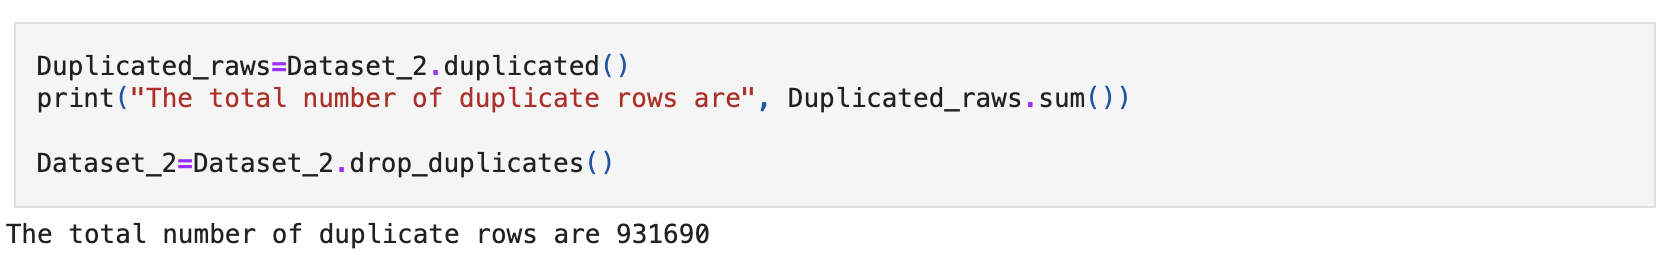
\includegraphics[scale=0.25]{Figures/duplicate.png}
    \end{figure}
\end{columns}
\vspace{0.3cm}
\begin{columns}
    \column{0.5\textwidth}
    \textbf{Deleting Rows with Null Values}
    \begin{itemize}
         \item We dropped all rows containing null values in some column.
     \end{itemize}

    \column{0.5\textwidth}
    \begin{figure}
        \centering
        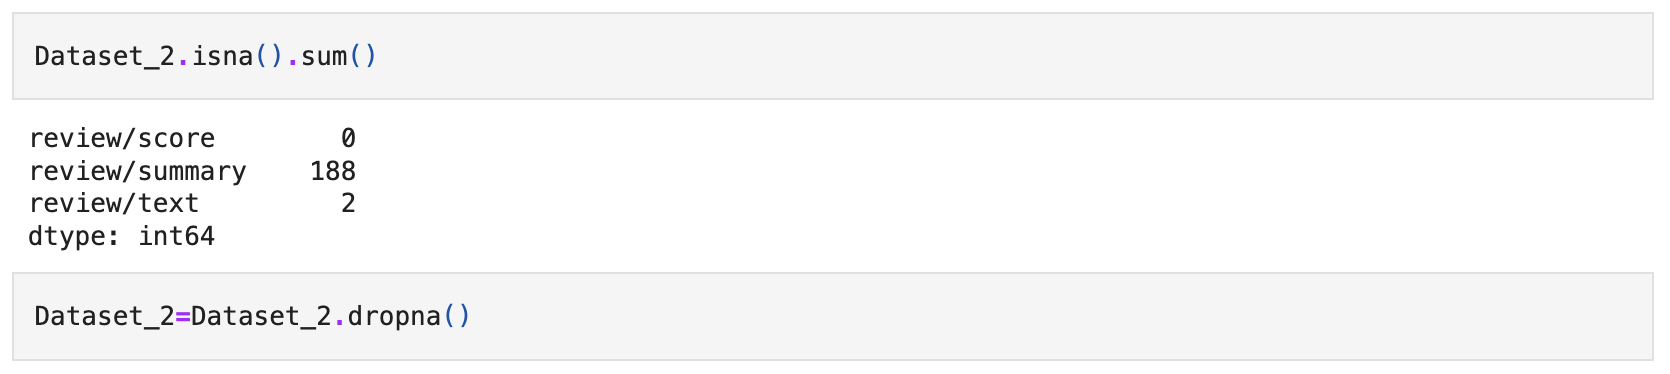
\includegraphics[scale=0.25]{Figures/null_values.png}
    \end{figure}
\end{columns}

}
\end{frame}

%~~~~~~~~~~~~~~~~~~~~~~~~~~~~~~~~~~~~~~~~~~~~~~~~~~~~~~~~~~~~~~~~~~~~~~~~~
\begin{frame}{Text Cleaning}
\framesubtitle{HLT Project: Data Cleaning}
{\small 

\begin{itemize}
    \item Defined a \texttt{Clean} \texttt{Text} function:
    \begin{enumerate}
        \item capable of eliminating special characters in the text.
        \item switching all uppercase letters to lowercase letters.
    \end{enumerate}
    \item Part of our model will be a pretrained transformer that works only with lowercase letters.
\end{itemize}

\begin{figure}
    \centering
    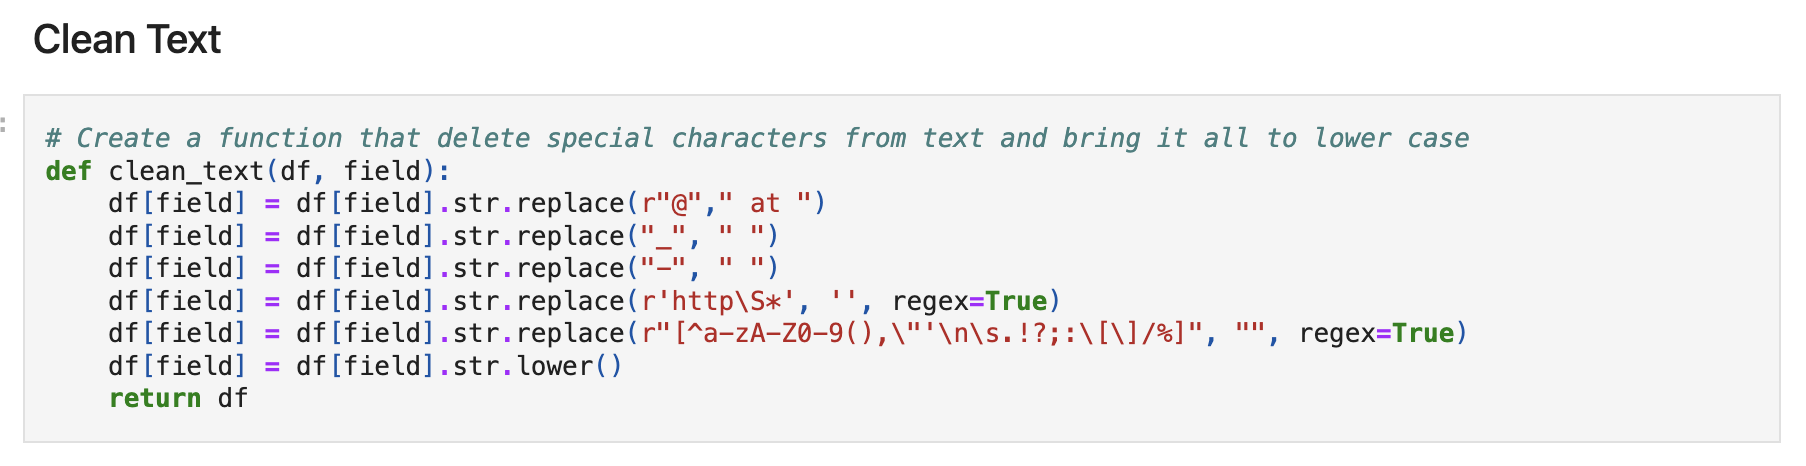
\includegraphics[scale=0.4, trim=0 0 0 1cm]{Figures/clean_text.png}
\end{figure}

\vspace{-0.5cm}
\begin{itemize}
    \item Applied this function to both datasets.
\end{itemize}
}
\end{frame}

%~~~~~~~~~~~~~~~~~~~~~~~~~~~~~~~~~~~~~~~~~~~~~~~~~~~~~~~~~~~~~~~~~~~~~~~~~~~~~~~~~~~~~~~~
%~~~~~~~~~~~~~~~~~~~~~~~~~~~~~~~~~~~~~~~~~~~~~~~~~~~~~~~~~~~~~~~~~~~~~~~~~~~~~~~~~~~~~~~~
\section{Data Analysis}

%~~~~~~~~~~~~~~~~~~~~~~~~~~~~~~~~~~~~~~~~~~~~~~~~~~~~~~~~~~~~~~~~~~~~~~~~~
\begin{frame}{Sentiment's Labels Distribution}
\framesubtitle{HLT Project: Data Analysis}
{\small 

\begin{itemize}
    \item The first thing we did is to see how the labels were distributed.
\end{itemize}
\vspace{-0.2cm}
\begin{columns}
    \column{0.5\textwidth}
    \center
    \textbf{Dataset\_1}
    \begin{figure}
        \centering
        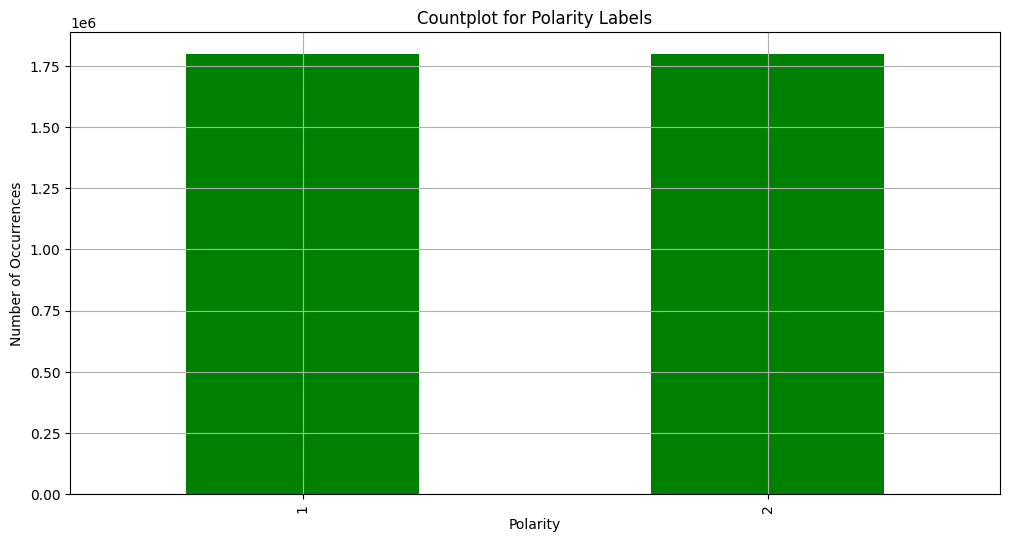
\includegraphics[scale=0.23]{Figures/fig1.png}
    \end{figure}
    \vspace{-0.2cm}
    \begin{itemize}
        \item The labels in the first dataset are already balanced.
    \end{itemize}
    
    \column{0.5\textwidth}
    \center
    \textbf{Dataset\_2}
    \begin{figure}
        \centering
        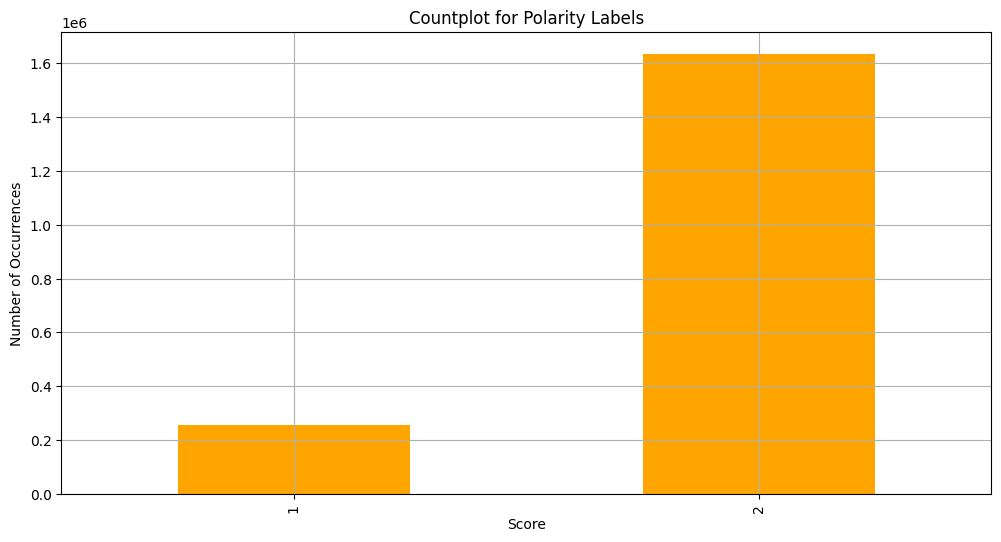
\includegraphics[scale=0.23]{Figures/fig3.png}
    \end{figure}
    \vspace{-0.2cm}
    \begin{itemize}
        \item In the second dataset we have many more positive reviews (about 85\% positive).
    \end{itemize}
    
\end{columns}

}
\end{frame}

%~~~~~~~~~~~~~~~~~~~~~~~~~~~~~~~~~~~~~~~~~~~~~~~~~~~~~~~~~~~~~~~~~~~~~~~~~
\begin{frame}{WordClouds}
\framesubtitle{HLT Project: Data Analysis}
{\small 

\begin{itemize}
    \item The second analysis concerns the most frequently used words in the datasets.
    \item Used the library \texttt{WordCloud} and defined a function \texttt{wordcloud\_fun}.
\end{itemize}

\begin{figure}
    \centering
    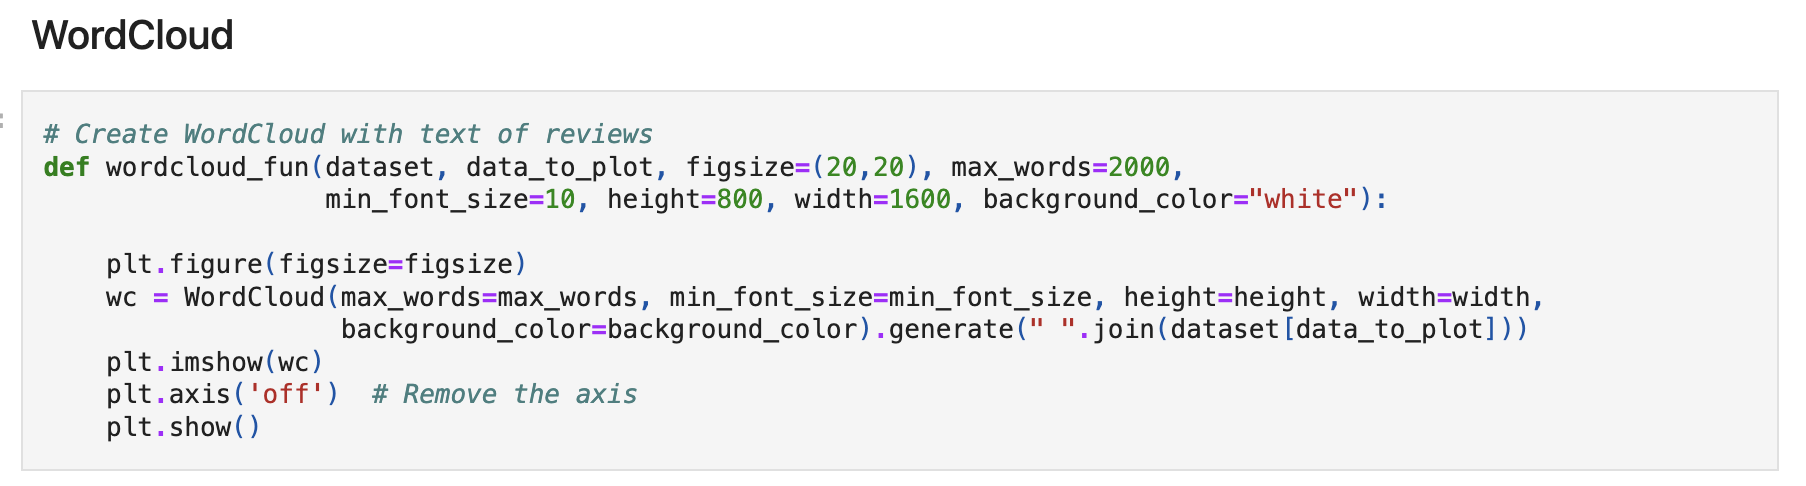
\includegraphics[scale=0.4]{Figures/wordcloud_fun.png}
\end{figure}

\begin{itemize}
    \item Searched for the most significant words by dividing texts with negative and those with positive reviews.
\end{itemize}

}
\end{frame}

%~~~~~~~~~~~~~~~~~~~~~~~~~~~~~~~~~~~~~~~~~~~~~~~~~~~~~~~~~~~~~~~~~~~~~~~~~
\begin{frame}{WordClouds}
\framesubtitle{HLT Project: Data Analysis}
{\small

\begin{columns}
    \column{0.3\textwidth}
    \center
    \textbf{WordClouds on Reviews}
    
    \column{0.35\textwidth}
    \center
    \texttt{Polarity=1}
    \begin{figure}
        \centering
        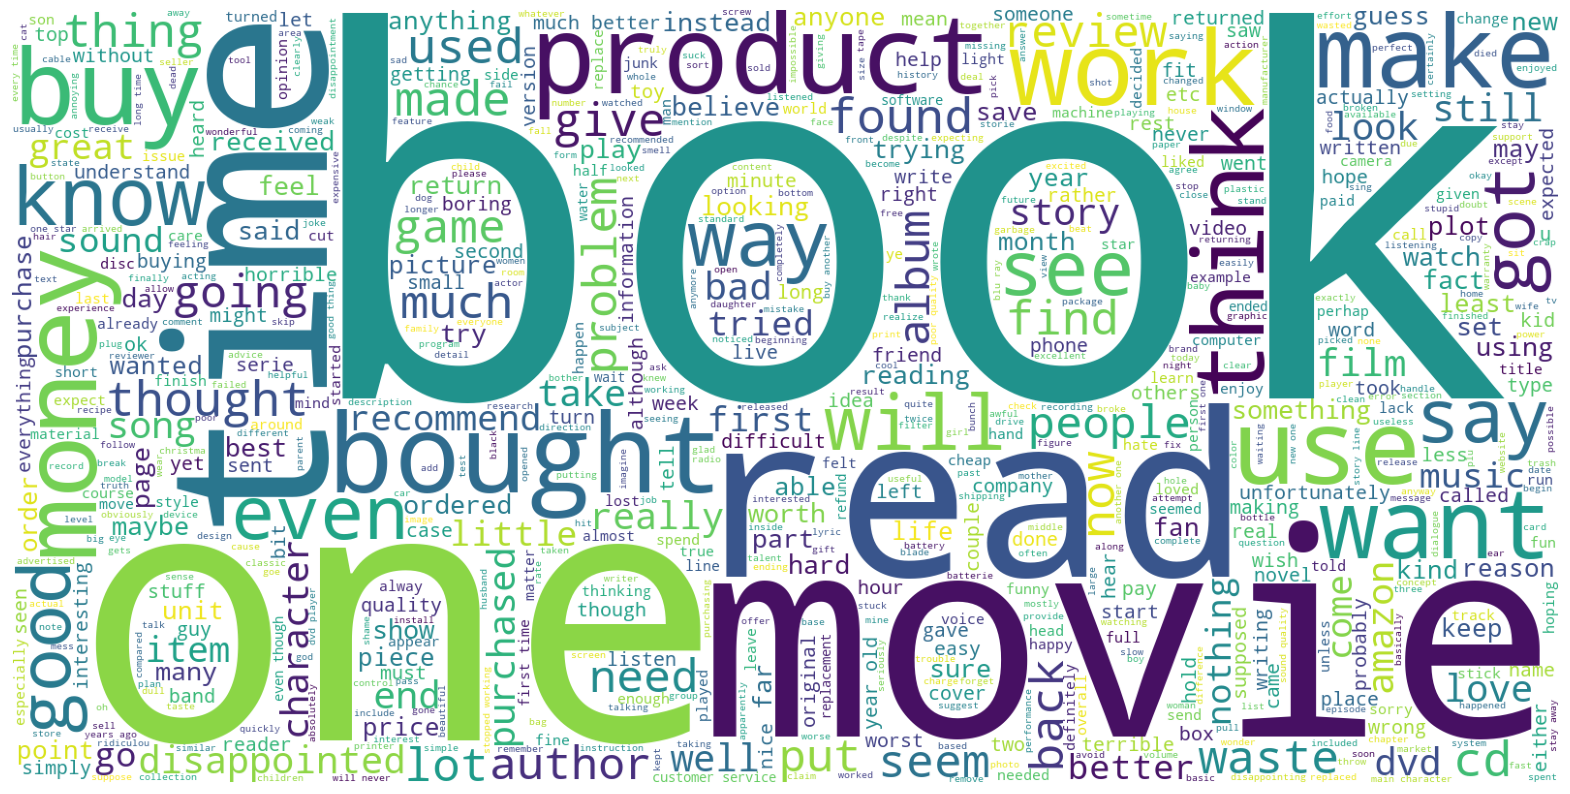
\includegraphics[scale=0.12, trim=0 0 0 1cm]{Figures/wordcloud_review1.1.png}
    \end{figure}

    \column{0.35\textwidth}
    \center
    \texttt{Polarity=2}
    \begin{figure}
        \centering
        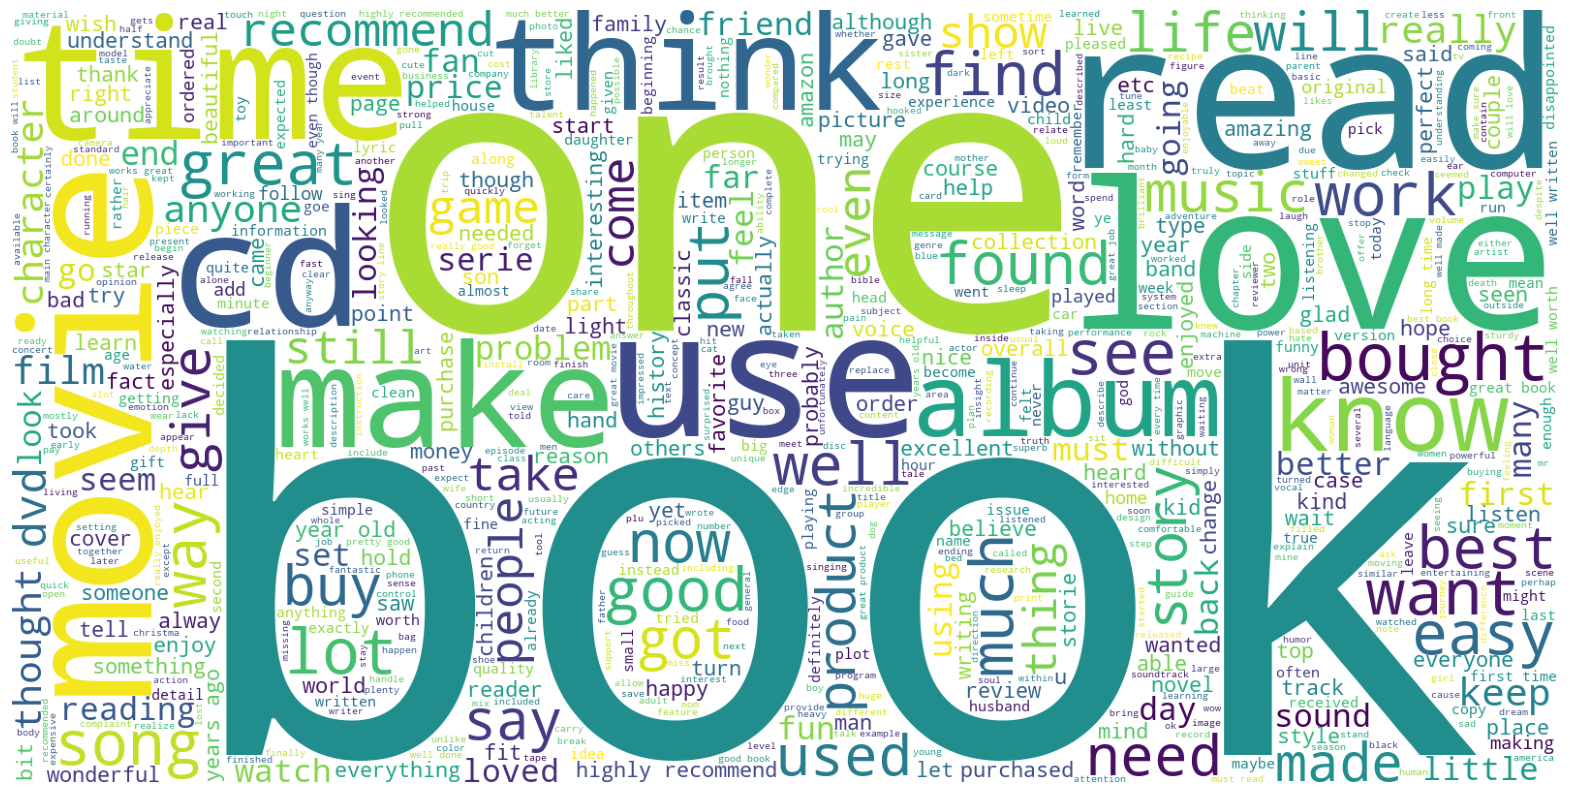
\includegraphics[scale=0.12, trim=0 0 0 1cm]{Figures/wordlcloud_review1.2.png}
    \end{figure}
\end{columns}

\begin{columns}
    \column{0.3\textwidth}
    \center
    \textbf{WordClouds on Titles}
    
    \column{0.35\textwidth}
    \begin{figure}
        \centering
        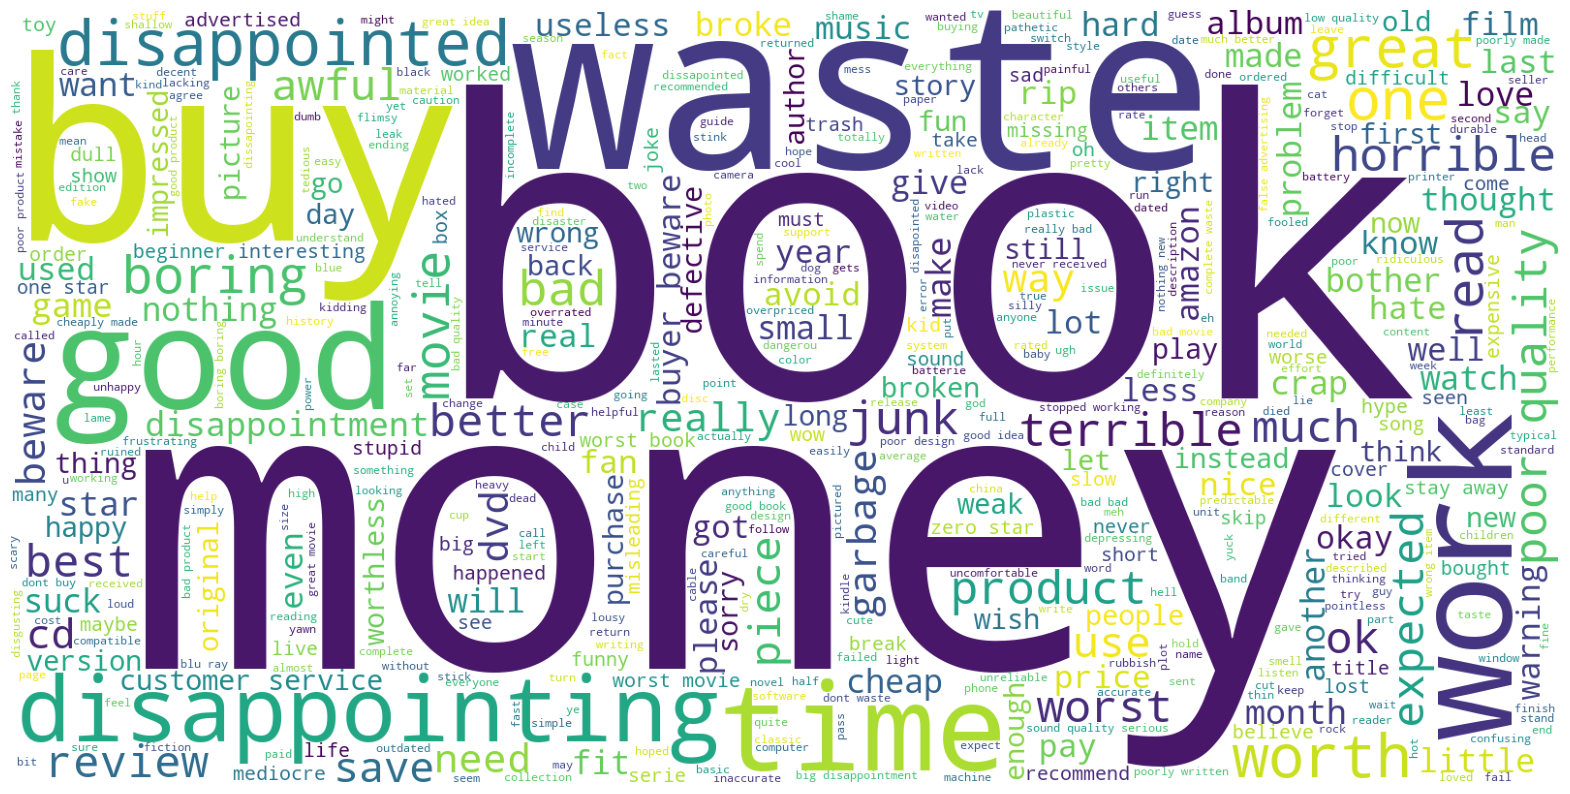
\includegraphics[scale=0.12, trim= 0 0 0 0cm]{Figures/wordcloud_title1.1.png}
    \end{figure}

    \column{0.35\textwidth}
    \begin{figure}
        \centering
        
\includegraphics[scale=0.12]{Figures/wordcloud_title1.2.png}
    \end{figure}
\end{columns}
}
\end{frame}

%~~~~~~~~~~~~~~~~~~~~~~~~~~~~~~~~~~~~~~~~~~~~~~~~~~~~~~~~~~~~~~~~~~~~~~~~~
\begin{frame}{Lenght of Text}
\framesubtitle{HLT Project: Data Analysis}
{\small 

\vspace{-0.3cm}
\begin{columns}
\column{0.5\textwidth}
\begin{itemize}
    \item The last analysis concerns the length of text in reviews and titles.
    \item Considered the length of a title as the number of words in the title.
    \item Printed histograms and box plots to study its distribution.
\end{itemize}

\column{0.5\textwidth}
\begin{figure}
    \centering
    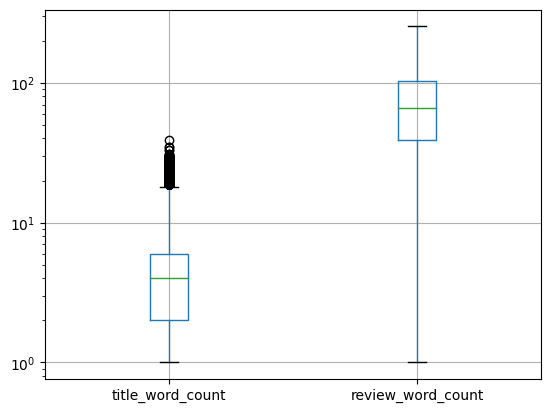
\includegraphics[scale=0.3]{Figures/boxplot2.png}
\end{figure}
\end{columns}

\vspace{-0.4cm}
\begin{columns}
    \column{0.5\textwidth}
    \begin{figure}
        \centering
        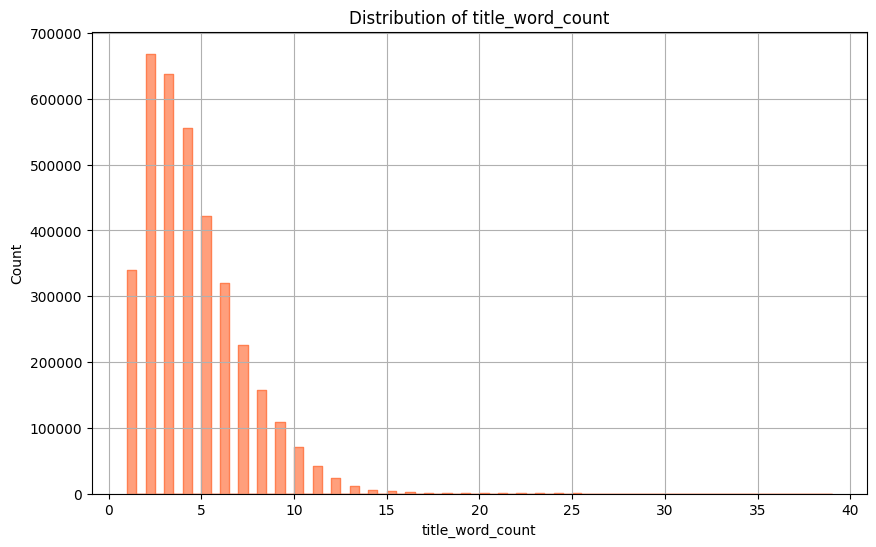
\includegraphics[scale=0.23]{Figures/distribution1.1.png}
    \end{figure}

    \column{0.5\textwidth}
    \begin{figure}
        \centering
        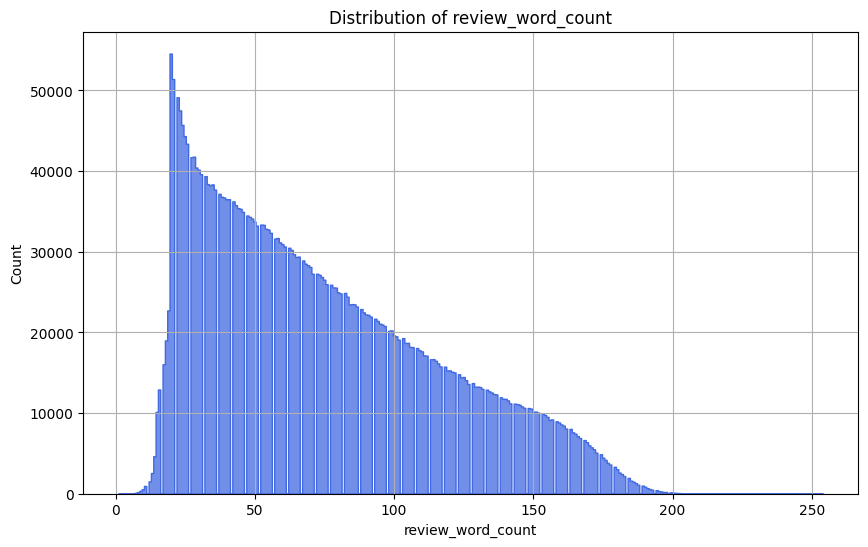
\includegraphics[scale=0.23]{Figures/distribution1.3.png}
    \end{figure}
\end{columns}
}
\end{frame}

%~~~~~~~~~~~~~~~~~~~~~~~~~~~~~~~~~~~~~~~~~~~~~~~~~~~~~~~~~~~~~~~~~~~~~~~~~
\begin{frame}{Lenght of Text}
\framesubtitle{HLT Project: Data Analysis}
{\small 

\begin{itemize}
    \item At this point we came up with a question:
    \begin{center}
        {\footnotesize \textit{"Is there a correlation between the length of reviews (or titles) and whether they are positive or not?"}}
    \end{center}
    \item Again printed out histograms to try to give us an answer.
\end{itemize}

\begin{columns}
    \column{0.5\textwidth}
    \begin{figure}
        \centering
        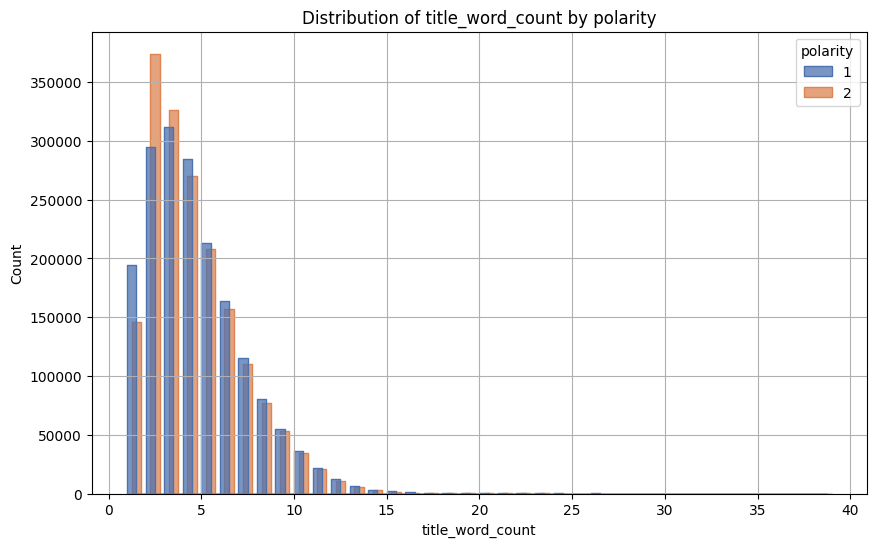
\includegraphics[scale=0.23]{Figures/distribution1.5.png}
    \end{figure}

    \column{0.5\textwidth}
    \begin{figure}
        \centering
        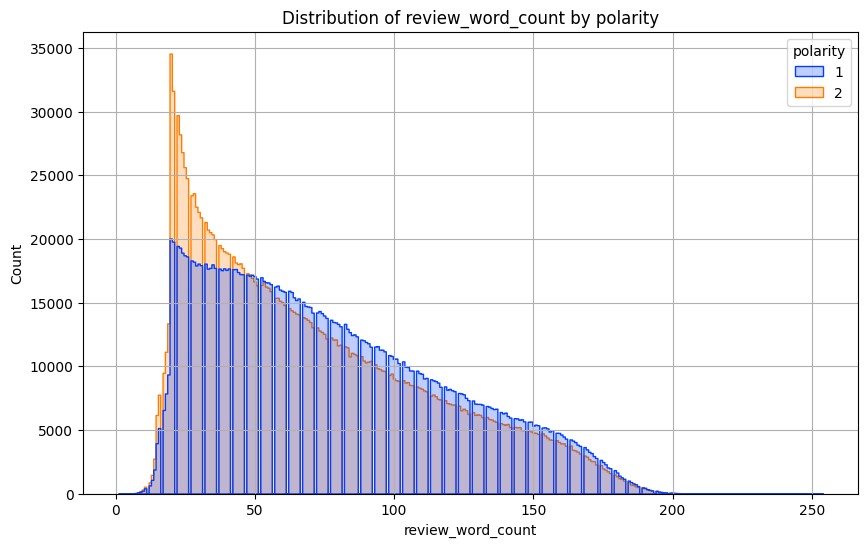
\includegraphics[scale=0.23]{Figures/distribution1.6.png}
    \end{figure}
\end{columns}

\begin{itemize}
    \item No. The distributions for positive and negative reviews are almost identical.
\end{itemize}

}
\end{frame}


%~~~~~~~~~~~~~~~~~~~~~~~~~~~~~~~~~~~~~~~~~~~~~~~~~~~~~~~~~~~~~~~~~~~~~~~~~
\begin{frame}{Bibliography}
\framesubtitle{HLT Project: Progress Update}

\begin{thebibliography}{9}
\setbeamertemplate{bibliography item}[text]
{\small

\bibitem{0} Angelido. "HLT-Sentiment-Analysis: Sentiment Analysis project repository." \emph{GitHub}. \href{https://github.com/Angelido/HLT-Sentiment-Analysis}{GitHub Repository.} (2024)

\bibitem{1} Wes McKinney. "Pandas: powerful Python data analysis toolkit." \emph{Python for High Performance and Scientific Computing. Vol. 14. No. 9.} \href{https://pandas.pydata.org/docs/}{Pandas Documentation.} (2011)

\bibitem{2} Andreas Mueller. "Word Cloud: A Command Line Interface for Creating Word Clouds." \emph{Journal of Open Source Software 3.26: 781}. \href{https://amueller.github.io/word_cloud/cli.html}{Word Cloud Command Line Interface.} (2018)

\bibitem{3} Michael Waskom et al. "Seaborn.histplot: Plot univariate or bivariate histograms to show distributions of datasets." \emph{The Journal of Open Source Software 6.60: 3021.} \href{https://seaborn.pydata.org/generated/seaborn.histplot.html}{Seaborn.histplot Documentation.} (2021)
}
\end{thebibliography}
    
\end{frame}

%~~~~~~~~~~~~~~~~~~~~~~~~~~~~~~~~~~~~~~~~~~~~~~~~~~~~~~~~~~~~~~~~~~~~~~~~~
\backmatter
\end{document}

